\section{Method: Learning and Compiling an Agent Safety Contract}\label{sec:method}
\system{} takes an instrumentable LLM agent $A$, a labeled ground-truth dataset $\mathcal{D}$ of agent trajectories, and a natural-language policy $P$ that summarizes this experience as inputs, and synthesizes a contract $C$ without a pre-existing specification. As outlined in Figure~\ref{fig:workflow_overview}, the method comprises (1) policy-guided abstraction of agent executions into events, (2) active learning of a permissible-behavior DFA with $L^*$, and (3) compilation into AgentSpec's trigger--check--enforce interface. The distinction between \emph{observing what an agent did} and \emph{judging whether it was permitted} is maintained throughout: an execution produces evidence, whereas a human or LLM expert supplies the policy judgment.

\begin{figure*}[t]
\centering
% trim removes the figure's old footnote line, which stated the previous guarantee; the caption now states it
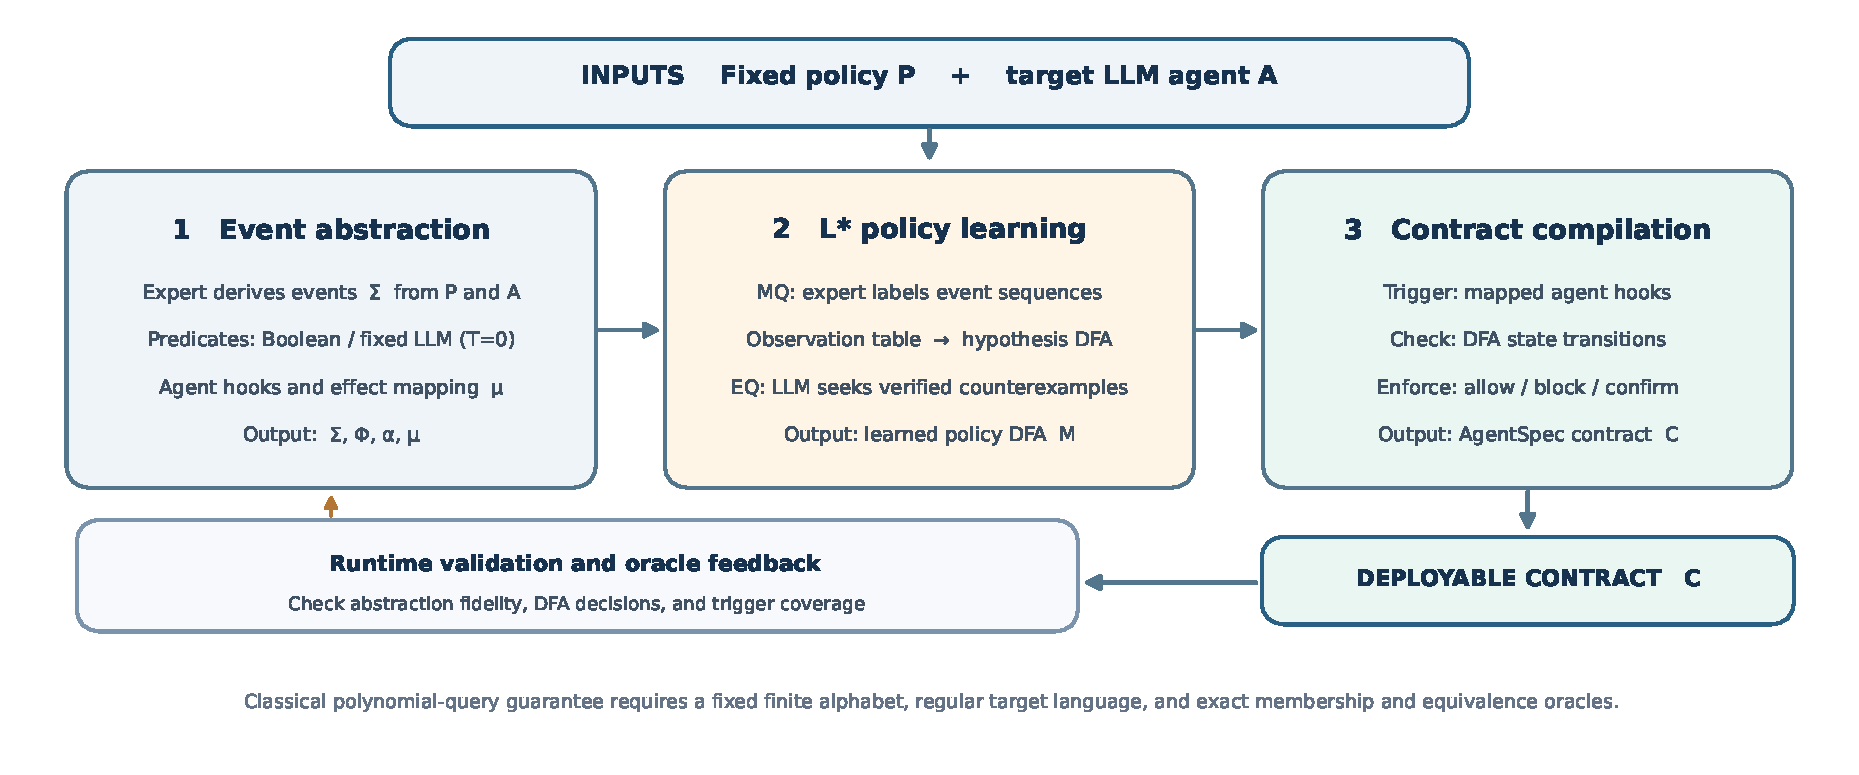
\includegraphics[width=0.94\textwidth,trim=0 52bp 0 0,clip]{figures/workflow_overview.pdf}
\caption{\system{} synthesizes an AgentSpec contract $C$ from an agent $A$, a policy $P$, and a labeled dataset $\mathcal{D}$. Agent-level instrumentation and expert-defined predicates produce ordered events over a fixed alphabet $\Sigma$. An $L^*$ learner answers membership queries from the dataset's labels where they apply and otherwise from an LLM that reads the policy, and refines its candidate DFAs with counterexamples: labeled trajectories on which the hypothesis is wrong. Event-to-hook mappings supply Trigger, the learned DFA supplies Check, and pre-effect mediation supplies Enforce. With correct labels and an LLM that is correct where the labels are silent, the learned DFA agrees with the whole dataset after at most $N-1$ counterexamples, and it is exact if the dataset is complete (Theorem~\ref{thm:exact}); exact enforcement additionally needs sufficient predicates and faithful interception (Corollary~\ref{cor:enforce}).}
\Description{Three phases: event abstraction from policy and instrumented agent, L-star learning with membership and counterexample queries, and compilation to AgentSpec trigger, check and enforce.}
\label{fig:workflow_overview}
\end{figure*}

\subsection{Phase 1: From Agent Execution to Event Streams}\label{sec:abstraction}
\paragraph{Selecting the observable events.}
A human or LLM expert examines $P$, the agent's tool schemas and workflows, and the available instrumentation points. It selects a finite alphabet $\Sigma$ of \emph{policy-relevant effects}, together with recognition predicates $\Phi$. A symbol is distinguished by the effect and policy-relevant context, not by the particular tool that produces it. The expert also specifies an event-to-hook mapping $\mu$, which identifies where each effect can be observed and, when consequential, intercepted before execution. The alphabet, predicates, and their implementations are fixed for a learning run; discovering that this abstraction is insufficient is reported as a limitation rather than silently changing the alphabet inside classical $L^*$.

\paragraph{Collecting and normalizing observations.}
Instrumentation at the agent's decision, tool-call, result, and state-update boundaries collects an ordered concrete trajectory $z=(o_1,\ldots,o_m)$, where each $o_i$ is an observation record. Records contain the proposed operation and its arguments, the correlated outcome, and the context needed to establish its actual policy-relevant effect. A proposal alone is not treated as a committed effect: failed or blocked calls do not emit the successful-effect symbol. If a tool invocation has several relevant effects, normalization yields separate, causally ordered records. LLM reasoning and other observations may contribute context without themselves producing an alphabet symbol. This normalization prevents, for instance, a failed public-link request from being confused with successful public disclosure.

\paragraph{Predicate-based event extraction.}
For each normalized record $o_i$, the recognizer evaluates $\Phi$ against $o_i$ and the relevant preceding context $h_i$. It emits either an event from $\Sigma$ or $\varepsilon$ (no policy-relevant event):
\[
 e_i=\operatorname{Recognize}_{\Phi}(o_i,h_i)
 \in\Sigma\cup\{\varepsilon\}.
\]
The context $h_i$ can include the current staging-slot contents, file sensitivity, effective link audience, and earlier tool outcomes, but is restricted to information available at the relevant observation point. The abstraction $\alpha$ concatenates the nonempty emissions in execution order:
\[
 \alpha(z)=e_1e_2\cdots e_m\in\Sigma^*,
\]
where $\varepsilon$ contributes no symbol. In the file-sharing example of Section~\ref{sec:motivating-example}, a successful confidential staging call emits $c$, replacement by a nonconfidential file emits $n$, and creation of a public link to the active staging slot emits $p$. Thus the executed sequence ``stage confidential, replace with normal, share publicly'' yields $\alpha(z)=cnp$ rather than $cp$. The replacement is a semantic effect established by the tool outcome, not guessed from the agent's stated intention.

\begin{table}[t]
\caption{Event extraction for the single-slot sharing agent. Only established effects emit events.}
\label{tab:event-extraction}
\centering\small
\begin{tabular}{p{0.47\columnwidth}p{0.39\columnwidth}}
\toprule
Observed outcome & Recognition and emission\\
\midrule
Stage confidential file successfully & Confidential payload $\rightarrow c$\\
Stage nonconfidential file successfully & Nonconfidential payload $\rightarrow n$\\
Create public link to active slot & Public audience $\rightarrow p$\\
Share request fails or is blocked & No committed effect $\rightarrow\varepsilon$\\
\bottomrule
\end{tabular}
\end{table}

Recognition predicates may be Boolean programs over structured fields or semantic classifiers implemented by a pinned LLM with a fixed prompt, output schema, and temperature zero. Repeated outputs for canonicalized inputs are cached. This improves repeatability, but neither temperature zero nor caching proves correct event classification. When the available evidence does not determine an event, the result is marked \texttt{unknown} and is not silently converted to $\varepsilon$. Before learning, sampled concrete traces are reviewed to check whether the abstraction preserves the policy distinctions needed for membership judgments. In particular, different concrete trajectories mapped to the same word must not have contradictory validated policy labels. A confirmed contradiction calls for expert review of the predicates or event meanings; abstraction refinement is outside the fixed-alphabet learning guarantee considered here.

\paragraph{Observations versus proposed effects.}
The same recognition rules support two execution phases. \emph{During learning}, $\alpha$ extracts events from successful effects observed in an isolated test environment. \emph{At deployment}, the trigger uses $\mu$ to recognize a proposed effect \emph{before commitment} and asks the monitor whether the corresponding event would be allowed. Only after the operation succeeds is the state transition committed. Proposed and observed effects must be reconciled; an unexpected or unclassifiable outcome requires a conservative fallback. This separation makes it possible to learn from real execution evidence while enforcing before an unsafe effect occurs.

\subsection{Phase 2: Active Learning of the Permissible Language}\label{sec:lstar}
\paragraph{Membership: labels first, then the policy.}
For a word $w\in\Sigma^*$, the ideal membership-query oracle answers $\operatorname{MQ}(w)=1$ iff $w\in L_G$, the ground-truth language of Section~\ref{sec:problem}. \system realizes it with two teachers. Before learning, the recognizer maps every trajectory of $\mathcal{D}$ to its word $\alpha(z)$, and the labels are entered into the answer cache under prefix closure: the word of a compliant trajectory and all its prefixes are members, and the word of a violating trajectory and all its extensions are non-members. Words determined both ways are collisions and are not entered. A membership query is then answered from the cache when the labels determine the word, so the labels always win. Only the remaining words reach an LLM with a pinned configuration, which reads the policy $P$, the event definitions and the sequence, and answers whether the sequence is acceptable. These are the words the data cannot settle: prefixes of violating trajectories, sequences that no trajectory contains, and words that no agent has realized yet. Here the policy is what generalizes the experience. If the LLM cannot decide, the query remains unresolved instead of receiving a fabricated label. Answers are cached with their provenance, label or LLM. For every word that the labels determine, \system also asks the LLM once, as a diagnostic: these answers are never used for learning, but their disagreements with the labels show where the policy does not summarize the experience. Theorem~\ref{thm:exact} assumes that the LLM is correct off the dataset (A3); Section~\ref{sec:rq2} measures how closely LLM judges meet that assumption.

\paragraph{Observation table and hypotheses.}
The $L^*$ learner~\cite{angluin1987learning} maintains a prefix set $S$, a set of distinguishing suffixes $E$, and a table $T$ of membership answers. Initially $S=E=\{\varepsilon\}$, where $\varepsilon$ is the empty word. For the one-event extensions $S\Sigma=\{sa\mid s\in S,a\in\Sigma\}$, the table contains
\[
 T(se)=\operatorname{MQ}(se),\quad
 s\in S\cup S\Sigma,\quad e\in E.
\]
The row $\operatorname{row}(s)=(T(se))_{e\in E}$ describes how history $s$ behaves under the tested continuations. The table is \emph{closed} when every row in $S\Sigma$ equals a row in $S$; it is \emph{consistent} when equal rows in $S$ remain equal after appending any alphabet event. A closure failure adds a representative history to $S$, whereas a consistency failure adds a distinguishing suffix to $E$. The learner obtains missing membership answers and repeats these steps until the table is closed and consistent. It then constructs a hypothesis DFA $\widehat M$ with one state per distinct row, transitions induced by one-event extensions, and accepting states given by membership of the corresponding histories.

For the alphabet $\Sigma=\{c,n,p\}$ of Section~\ref{sec:motivating-example}, the initial queries $\operatorname{MQ}(\varepsilon)$, $\operatorname{MQ}(c)$, $\operatorname{MQ}(n)$, and $\operatorname{MQ}(p)$ all return 1. Hence the first hypothesis accepts every word. The verified counterexample $cp$, with $\operatorname{MQ}(cp)=0$, exposes its error. Adding the suffix $p$ distinguishes the empty history from $c$, since $\operatorname{MQ}(p)=1$ but $\operatorname{MQ}(cp)=0$. Additional queries such as $\operatorname{MQ}(cnp)=1$ and $\operatorname{MQ}(ncp)=0$ establish how replacement staging affects future public sharing. Repeated table refinement can recover the three policy states in Figure~\ref{fig:sharing-dfa}; the developer does not provide their transition rules.

\paragraph{Equivalence checking against the dataset.}
An exact equivalence query asks whether the current DFA is correct and, if not, returns a counterexample word. No oracle answers it, and \system does not ask an LLM to: an LLM able to certify equivalence would make learning unnecessary (Section~\ref{sec:problem}). Instead, the labeled dataset answers it, so that every correction to the contract is backed by real feedback from the world. Each round replays the abstracted dataset through $\widehat M$, shortest words first, and returns the word $\alpha(z)$ of the first disagreement, a labeled trajectory $(z,y)$ with $\widehat M(\alpha(z))\neq y$, where $\widehat M(w)\in\{0,1\}$ is the hypothesis's acceptance decision. Since the membership teacher answers this word with its label, the counterexample is valid by construction; disagreements on collision words are reported and skipped. In the running example, labeled trajectories whose words are $cp$, $cnp$, and $ncp$ respectively challenge unsafe acceptance, erroneous over-restriction, and the effect of staging order. Because the label of a violating trajectory concerns the whole trajectory, its word may be longer than the shortest violating prefix; $L^*$'s counterexample processing adds the word's prefixes to the table, and membership queries locate the violation.

\paragraph{Learning loop and stopping condition.}
Each counterexample is returned to $L^*$, which refines its observation table and constructs another hypothesis. Learning stops when a hypothesis agrees with every labeled trajectory of $\mathcal{D}$ outside collisions, when an unresolved membership query suspends it, or when the budget is exhausted. The number of counterexamples never exceeds the number of distinct words in the dataset (Theorem~\ref{thm:exact}(a)). A returned DFA is \emph{dataset-consistent} (Theorem~\ref{thm:exact}(b)); it is exact on realizable words only if the dataset is complete (Theorem~\ref{thm:exact}(c)), which \system does not assume.

\paragraph{Query cost.}
Under (A2) and (A3), learning uses at most $O(|\Sigma|(B+1)N^2)$ membership queries, where $B$ is the length of the longest word in the dataset, and at most $N-1$ counterexamples, as in classical $L^*$~\cite{angluin1987learning}. Only the queries that the labels do not determine reach the LLM, plus one diagnostic query per distinct dataset word. Each round replays the dataset once, in time linear in its total length. These bounds count abstract queries. They do not bound LLM tokens or human review time, which Section~\ref{sec:eval} reports.

\subsection{Phase 3: DFA-to-AgentSpec Compilation}\label{sec:compile}
\paragraph{Trigger from concrete event mappings.}
The learned DFA determines which abstract event transitions may matter for the policy; $\mu$ maps those symbols back to concrete agent-tool and state-update hooks. The compiler instruments all events needed to maintain the DFA state, not only events that are immediately dangerous. Consequential calls whose proposed effects may enter a rejecting state must be intercepted before their effects commit. If multiple tools implement the same effect, all relevant implementations must be mapped. This is an agent-level integration contract, not an assumption of OS-wide interception.

\paragraph{Check from the learned DFA.}
For the learned hypothesis $\widehat M=(Q,\Sigma,\delta,q_0,F)$ defined in Section~\ref{sec:problem}, the monitor starts in state $q_0$. For a proposed event $e\in\Sigma$ at current state $q\in Q$, it computes $q'=\delta(q,e)$. For a prefix-closed hypothesis language, a transition to $q'\notin F$ is rejected before execution; otherwise, execution may proceed. The compiler checks this prefix-closure condition before claiming language-equivalent enforcement; a candidate that fails the check requires further learning or an explicitly reported conservative restriction. A successful effect commits $q'$, while a failed or blocked effect leaves the monitored policy state unchanged. Concurrent calls must be serialized or reconciled using a causally correct order. If the effect cannot be classified reliably before execution, the monitor follows a conservative fallback rather than allowing an unmonitored transition.

\paragraph{Enforce and validate.}
AgentSpec performs \texttt{ALLOW} or \texttt{BLOCK} according to the DFA check. A \texttt{CONFIRM} action or remediation is included only if a policy-defined procedure specifies its meaning and subsequent state effects; user confirmation alone is not assumed to turn a forbidden disclosure into a permissible one. The resulting contract is $C=\operatorname{Compile}(\widehat M,\alpha,\mu)$. Compilation is \emph{faithful} when the monitor accepts exactly the abstract words accepted by $\widehat M$ over the instrumented boundary. We test this property through transition-level differential replay and end-to-end interception, separately from the accuracy of the learned DFA and the adequacy of the abstraction. In particular, an accurate DFA cannot compensate for a missed trigger or an event classified after an irreversible effect.
